\documentclass[sigconf]{acmart}

\usepackage{booktabs} % For formal tables

\usepackage{pifont}
\usepackage{listings}
\lstdefinelanguage{potc}{
  morekeywords={parameter,real,type,function,peratom,atom,sum,neighbors,energy,spline,cos,energy,atom_type,all_atoms,implicit,piecewise,sin,cos,exp,file,distance}
}
\usepackage{pgfplots}
\usetikzlibrary{calc,decorations,angles,quotes,external,arrows.meta}

\definecolor{rwthdarkblue}{RGB}{0,84,159}
\definecolor{rwthlightblue}{RGB}{142,186,229}
\definecolor{rwthdarkgray}{RGB}{100,101,103}
\definecolor{rwthlightgray}{RGB}{236,237,237}

\definecolor{rwthmagenta}{RGB}{227,0,102}
\definecolor{rwthyellow}{RGB}{255,237,0}
\definecolor{rwthpetrol}{RGB}{0,97,101}
\definecolor{rwthturquoise}{RGB}{0,152,161}
\definecolor{rwthgreen}{RGB}{87,171,39}
\definecolor{rwthmaygreen}{RGB}{189,205,0}
\definecolor{rwthorange}{RGB}{246,168,0}
\definecolor{rwthred}{RGB}{204,7,30}
\definecolor{rwthbordeauxred}{RGB}{161,16,53}
\definecolor{rwthviolet}{RGB}{97,33,88}
\definecolor{rwthpurple}{RGB}{122,111,172}

\setcopyright{none}

%Conference
\acmConference[ACM SRC/SC18]{ACM Student Research Competition at SC17}{November 2018}{Dallas, Texas USA}
\acmYear{2018}

\begin{document}
\title{PotC: Many-body potential implementations \`a la carte}
\subtitle{Poster Summary}

\author{Markus H\"ohnerbach}
\affiliation{%
  \institution{RWTH Aachen University}
}
\email{hoehnerbach@aices.rwth-aachen.de}

\author{Paolo Bientinesi}
\authornote{Advisor}
\affiliation{%
  \institution{RWTH Aachen University}
}
\email{pauldj@aices.rwth-aachen.de}

\renewcommand{\shortauthors}{M. H\"ohnerbach et al.}

\maketitle

\section{Introduction}

Molecular dynamics simulations are a valuable tool in computational chemistry and materials science.
The atoms in these simulations move according to so-called potentials.
Often, these potentials are pair-wise and describe distance-dependent interactions.
However, some applications require many-body formulations, e.g. because of angle-dependent interactions.

Such potentials pose a number of challenges:
Small neighborhoods complicate vectorization;
redundant force expressions are tedious to manually derive;
the implementations are large, runtime-critical, and can not be broken into simpler ``kernels''.

Effectively, only the most popular many-body potentials are optimized---with major effort.

To tackle these issues, we introduce a DSL for MD potentials and a corresponding compiler to derive high-performance implementations.
Our goal is to centralize optimization knowledge for many-body potentials within the compiler, and unburden users from manual optimization and the derivation of forces.

\section{Molecular Dynamics}

Molecular dynamics potentials specify how atoms attract and repulse each other and account for the majority of the simulation runtime.
They are given as functions of all atom positions:
$$V(\mathbf{x}_1, \dots, \mathbf{x}_N).$$

And forces can be derived using
$$\mathbf{F}_i = -\nabla_{\mathbf{x}_i} V.$$

Simplest and most popular potential (pairwise) depends on distance:
$$V=\sum_i\sum_{j, r_{ij} < r_c} f(r_{ij}).$$

Many-body potentials are required to model some materials, and depend on more than just distance:
They can depend on the angles between three atoms, the ``twist'' (dihedral angle) between four atoms, some measure of bond-strength that depends on the local neighborhood, or some kind of per-atom embedding energy.

Fig.~\ref{fig:sel-pot} lists some potentials included with LAMMPS together with their approximate complexity using LOCs as well as (if available) their vectorized (USER-INTEL package) counterparts, which reuse code from the regular implementation.
For most listed potentials forces can not be computed from distances between atom pairs.

To illustrate, we fully define Tersoff potential (Fig.~\ref{fig:ma-ters}).

\begin{figure*}
\pgfplotsset{compat=1.11,
    /pgfplots/ybar legend/.style={
    /pgfplots/legend image code/.code={%
       \fill[##1,/tikz/.cd,yshift=-0.25em]
        (0cm,0cm) rectangle (0.4em,0.8em);},
   },
}
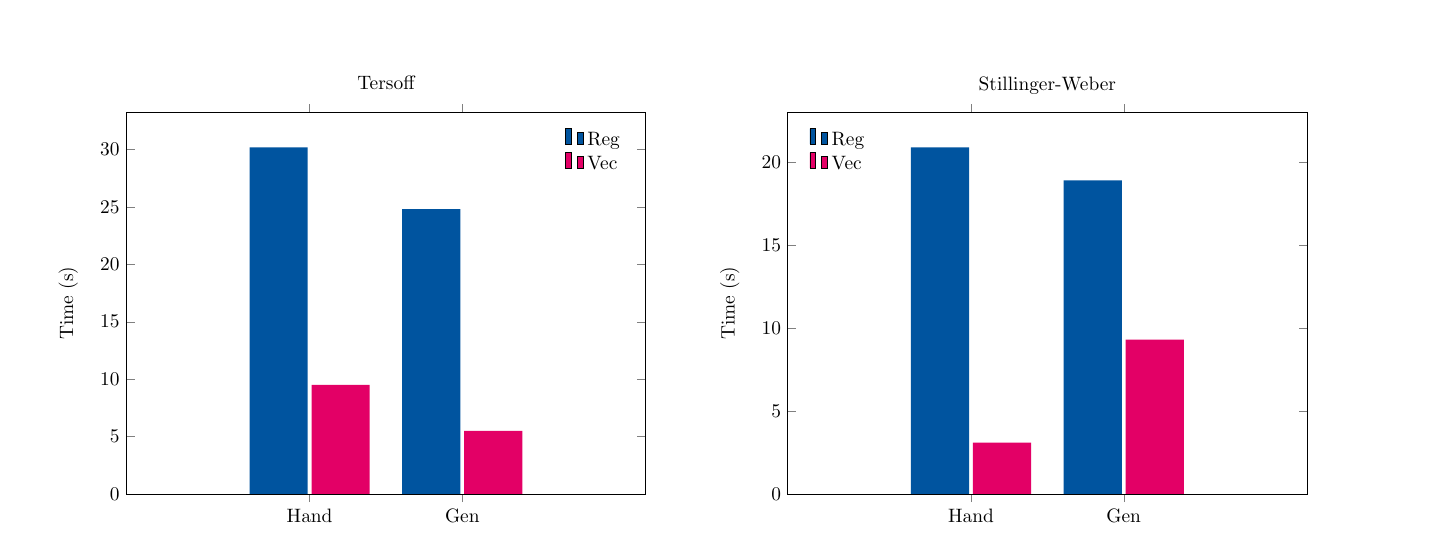
\begin{tikzpicture}[scale=0.7]
%\draw[gray] (0, 0) grid (25, 10);                                                                                                   
\node (t) at (6.5, 5.0) {};                                                                                                                  
\node (s) at (18.5, 5.0) {};                                                                                                                 
\begin{axis}[legend cell align=left,                                                                                                         
    legend pos=north east, 
    legend style={draw=none},
    ylabel={Time (s)},
    %label style={font=\footnotesize},                                                                                                        
    %tick label style={font=\tiny},                                                                                                           
    %x tick label style={font=\small},                                                                                                        
    y label style={at={(axis description cs:-0.08,.5)},anchor=south},                                                                        
    axis background/.style={fill=white},                                                                                                     
    legend style={fill=none},
    ybar, bar width=30pt,
    enlarge x limits=1.2,
    ymin=0,
    symbolic x coords={Hand, Gen},
    xtick={Hand, Gen},
    title={Tersoff\rule[-0.2\baselineskip]{0pt}{1\baselineskip}},
    at={(t)}, anchor=center,
    height=8.5cm, width=11cm
]
\addplot[draw=none, fill=rwthdarkblue] coordinates { (Hand, 30.2) (Gen, 24.8) };
\addplot[draw=none, fill=rwthmagenta]  coordinates { (Hand, 9.5) (Gen, 5.5) };
\legend{ Reg, Vec }
\end{axis}

\begin{axis}[legend cell align=left,
    legend pos=north west,
    legend style={draw=none},
    ylabel={Time (s)},
    %label style={font=\footnotesize},
    %tick label style={font=\tiny},
    %x tick label style={font=\small},
    y label style={at={(axis description cs:-0.08,.5)},anchor=south},
    axis background/.style={fill=white},
    legend style={fill=none},
    ybar, bar width=30pt,
    enlarge x limits=1.2,
    ymin=0,
    symbolic x coords={Hand, Gen},
    xtick={Hand, Gen},
    title={Stillinger-Weber},
    at={(s)}, anchor=center,
    height=8.5cm, width=11cm
]
\addplot[draw=none, fill=rwthdarkblue] coordinates { (Hand, 20.9) (Gen, 18.9) };
\addplot[draw=none, fill=rwthmagenta]  coordinates { (Hand, 3.1) (Gen, 9.3) };
\legend{ Reg, Vec }
\end{axis}
\pgfresetboundingbox
\path [use as bounding box] (0, 1) rectangle (25, 10);
\end{tikzpicture}
\caption{Performance results for two potentials. Handwritten implementation contained in LAMMPS vs automatically generated code, both either regular or vectorized.}\label{fig:perf}
\end{figure*}
\begin{figure}
\begin{center}
\begin{tabular}{llll}
\bfseries Name &\bfseries  LOC-R &\bfseries  LOC-O &\bfseries  Structure\\
LJ & 640 & +480 & {\small $\sum_i\sum_j f(i, j)$}\\
Stillinger-Weber & 600 & +1250 & {\small $\sum_i\sum_j\sum_k f(i,j,k)$}\\
EAM & 840 & +820 & {\small $\sum_i f(i, \sum_j g(i, j))$}\\
Tersoff & 800 & +1450 & {\small $\sum_i\sum_j f(i, j, \sum_k g(i, j, l)$}\\
MEAM & 890 & \ding{55}  & {\small $\sum_i f(i, \sum_j g(i, j))$}\\
ADP & 940  & \ding{55}  & too complex to show\\
BOP & 5950 & \ding{55}  & too complex to show\\
(AI)REBO & 4240 & +4550 & too complex to show\\
COMB3 & 3560   & \ding{55} & too complex to show\\
ReaxFF & 10880 & \ding{55} & too complex to show
\end{tabular}
\end{center}
LOC-R: Lines of code of the regular code.\\
LOC-O: Extra LOC in the optimized/vectorized code.
\caption{Selected Potentials from LAMMPS}
\label{fig:sel-pot}
\end{figure}

%\section{Motivation}
%
%Many-body potentials are complex to implement, and require large effort to optimize.
%Less popular potentials will likely never be optimized manually.
%
%
%And even if there is an implementation, it can be hard to assure that it is correct.
%
%
%To tackle these issues, this work introduces a Domain Specific Language for molecular dynamics potentials and a corresponding compiler to derive high performance implementations.

\begin{figure}
\begin{align*}
V &= \sum_i\sum_j f_C(r_{ij}) [ f_R(r_{ij}) + b_{ij} f_A(r_{ij}) ]\\
f_C(r) &= \begin{cases}
  0, & r < R - D\\
  \frac{1}{2} - \frac{1}{2}\sin(\frac{\pi}{2} (r - R) / D), & R - D < r < R + D\\
  1 & r > R + D
\end{cases}\\
f_R(r) &= A\exp(-\lambda_1 r)\\
f_A(r) &= -B\exp(-\lambda_2 r)\\
b_{ij} &= (1 + \beta^n\zeta_{ij}^n)^{1/(2n)}\\
\zeta_{ij} &= \sum_k f_C(r_{ik}) g(\theta_{jik}) \exp(\lambda_3^m (r_{ij} - r_{ik})^m)\\
g(\theta) &= \gamma (1 + c^2/d^2 - c^2/(d^2 + (\cos(\theta) - \cos(\theta_0))^2))\\
\end{align*}


Parameters: $R$, $D$, $A$, $\lambda_1$, $B$, $\lambda_2$, $\beta$, $n$, $\lambda_3$, $m$, $\gamma$, $c$, $d$, $\theta_0$.
\caption{The Tersoff potential specified using mathematical notation.}\label{fig:ma-ters}
\end{figure}

\section{Challenges}

Writing good optimized many-body potential implementations poses a number of challenges:

\begin{itemize}
\item One has to pick a vectorization strategy that is suitable to the (potentially very short) neighbor list lengths.
\item One has to reduce the amount of recalculation for the force computation.
\item Especially when vectorizing it is imperative to explore the possibility of reduced accuracy because it allows twice as wide vectors.
\item Vectorization of MD potentials has a number of idioms that need to be applied.
\end{itemize}

\section{Approach}

As indicated on the poster, the compiler performs four steps.

First, the input DSL is parsed, resulting in a ``functional'' representation of the potential energy (i.e. side effect free).
An excerpt of the DSL for the Tersoff potential (Fig.~\ref{fig:ma-ters}) can be found on the poster.

Second, the force derivation step adds the statements for force accumulation, transferring to an imperative representation.
It uses the adjoint-based approach well-known from the domain of Automatic Differentiation to do so.
It essentially ``interprets`` the functional representation and emits the corresponding code.

Third, optimizations are performed on the imperative representation as multiple passes.
Right now there are passes for inlining, loop and conditional fusion, dead code elimination, common subexpression elimination, arithmetic improvements (e.g. constant folding, $\sin$/$\cos$ laws), identification of identical values, and loop invariant code motion.
In the future, we plan to add improved common subexpression elimination, propagation of $0$, some kind of intermediate value caching, batching and accuracy reduction.
There exists rudimentary, buggy support for vectorization that will be improved further.

Last, the compiler generates source code that can be compiled into LAMMPS.
LAMMPS is a popular, extensible, open-source, highly scalable molecular dynamics code developed by Sandia National Labs.
It contains implementations for a number of many-body potentials, in various implementation variants (threaded, vectorized, GPU, \dots).
In addition LAMMPS provides benchmarks for all its potentials, which can be used to evaluate our results.

\section{Results}

We present preliminary results, since not all the planned optimizations are yet implemented (Fig.~\ref{fig:perf}).
We picked the potentials since they are popular, relatively simple and have both ``regular'' and ``vectorized'' implementations.
The performance of the generated code matches the handwritten implementation quite well, beating it in all cases but the vectorized Stillinger-Weber case which aggressively caches intermediate values across loops, an optimization that we do not support yet.

\section{Future Work}
The tool is currently far from complete.
In addition to implementing previously mentioned optimizations, we also want to add features that are not performance-related.
In particular, we want support more potentials by adding tabulated functions, FFI and searches through neighbor lists.
We are considering a LAMMPS/KOKKOS backend (GPU support) and a KIM API backend (better interoperability).
In principle, we could also perform other symbolic manipulations, e.g. calculate parameter derivatives, or accurate Hessians.

\section{Conclusion}
PotC can be a valuable tool for molecular dynamics software authors and users.
It allows them to quickly prototype novel potentials, test against a mechanical ``ground truth``, reach less popular potentials with optimizations, communicate potentials unambiguously, do symbolic manipulation of potentials (e.g. parameter derivatives or Hessians), and avoid writing redundant code and optimizing it by hand.

%\section{References}
%
%\bibliographystyle{ACM-Reference-Format}
%\bibliography{sample-bibliography}

\end{document}
